\documentclass{beamer}

% There are many different themes available for Beamer. A comprehensive
% list with examples is given here:
% http://deic.uab.es/~iblanes/beamer_gallery/index_by_theme.html
% You can uncomment the themes below if you would like to use a different
% one:
%\usetheme{AnnArbor}
%\usetheme{Antibes}
%\usetheme{Bergen}
%\usetheme{Berkeley}
%\usetheme{Berlin}
%\usetheme{Boadilla}
%\usetheme{boxes}
%\usetheme{CambridgeUS}
%\usetheme{Copenhagen}
%\usetheme{Darmstadt}
%\usetheme{default}
\usetheme{Frankfurt}
%\usetheme{Goettingen}
%\usetheme{Hannover}
%\usetheme{Ilmenau}
%\usetheme{JuanLesPins}
%\usetheme{Luebeck}
%\usetheme{Madrid}
%\usetheme{Malmoe}
%\usetheme{Marburg}
%\usetheme{Montpellier}
%\usetheme{PaloAlto}
%\usetheme{Pittsburgh}
%\usetheme{Rochester}
%\usetheme{Singapore}
%\usetheme{Szeged}
%\usetheme{Warsaw}

% Chinese display
\usepackage{CJKutf8}

% English? (cause Overleaf)
\usepackage[english]{babel}

% Flow Charts 
\usepackage{tikz}
\usetikzlibrary{shapes.geometric, arrows}
\tikzset{
	flowchartnode/.style = {minimum width=3cm, minimum height=1cm, text centered, draw=black},
	process/.style = {rectangle, flowchartnode, fill=orange!30},
	decision/.style = {diamond, flowchartnode, fill=green!30},
	io/.style = {trapezium, trapezium left angle=70, trapezium right angle=110, flowchartnode, fill=blue!30},
	line/.style = {draw, -latex'}
}

% Indexed letters inside circles
\newcommand\encircle[1]{%
  \tikz[baseline=(char.base)]{
  	\node[shape=circle,draw,inner sep=2pt] (char) {#1};}}

% Tab
\newcommand{\tab}[1]{\hspace{.1\textwidth}\rlap{#1}}

% Divider
\newcommand{\divider}[1]{\noindent\rule{.9\textwidth}{1pt}}

% Set caption with tiny size
\setbeamerfont{caption}{size=\tiny}

\addtobeamertemplate{navigation symbols}{}{%
    \usebeamerfont{footline}%
    \usebeamercolor[fg]{footline}%
    \hspace{1em}%
    \insertframenumber/\inserttotalframenumber
}
\setbeamercolor{footline}{fg=blue}
\setbeamerfont{footline}{series=\bfseries}

% Figure directory
\graphicspath{{fig/}{fig/scenario/}{fig/schemes/}{fig/protocol/}{fig/experiment/}}

% First page
\title[Oral Presentation]{Implementing Real-time POV for Cloud Storage by Replication and Voting}
\author[Wei-Chih Chien]{Advicer : Gwan-Hwan Hwang \texorpdfstring{\\ Student : Wei-Chih Chien}{}}
\institute[NTNU CSIE CCLAB]{NTNU CSIE CCLAB}
\date{2016.07}

% Start content
\begin{document}
% Chinese display
\begin{CJK}{UTF8}{bsmi}

\begin{frame}
  \titlepage
\end{frame}

\begin{frame}{Outline}
  \tableofcontents
\end{frame}

\section{Scenario}

\begin{frame}{Scenario}{Law Office}
	\begin{center}
		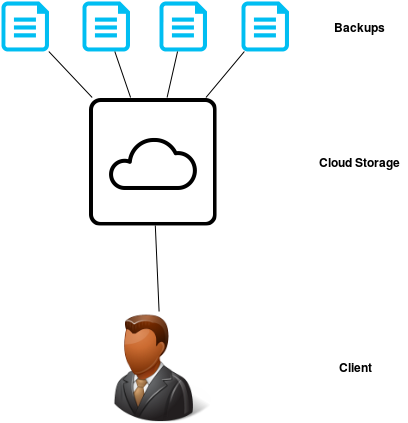
\includegraphics[height=.7\textheight]{Scenario1}
	\end{center}
\end{frame}

\begin{frame}{Scenario (CON'T)}{What if...}
	\begin{center}
		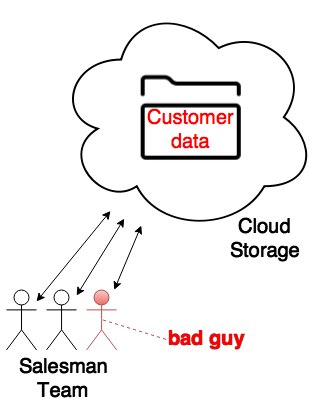
\includegraphics[height=.7\textheight]{Scenario2}\\
        \textcolor{blue}{Service Provider's Rollback Attack}
	\end{center}
\end{frame}

\begin{frame}{Scenario (CON'T)}
	\begin{center}
		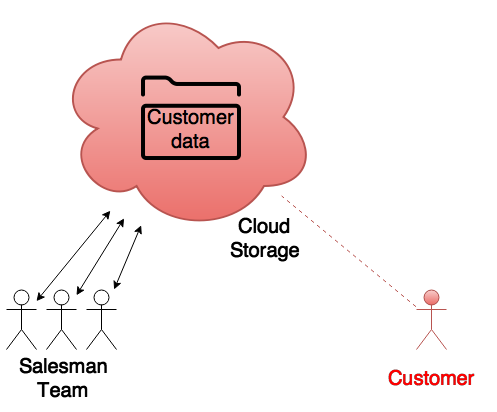
\includegraphics[height=.8\textheight]{Scenario3}
	\end{center}
\end{frame}

\begin{frame}{Scenario (CON'T)}
	\begin{center}
		\includegraphics[height=.7\textheight]{Scenario4}\\
        \textcolor{blue}{Obtaining Mutual Non-repudiation}
	\end{center}
\end{frame}
\section{Real-time Auditing Schemes}

\subsection{\small{Instant Auditing of Cloud Storage Access by Cache Partial Merkle tree}}
\begin{frame}{\normalsize{Instant Auditing of Cloud Storage Access by Cache Partial Merkle tree}}
{\tiny{2014 IEEE 6th International Conference on Cloud Computing Technology and Science}}
	\begin{center}
		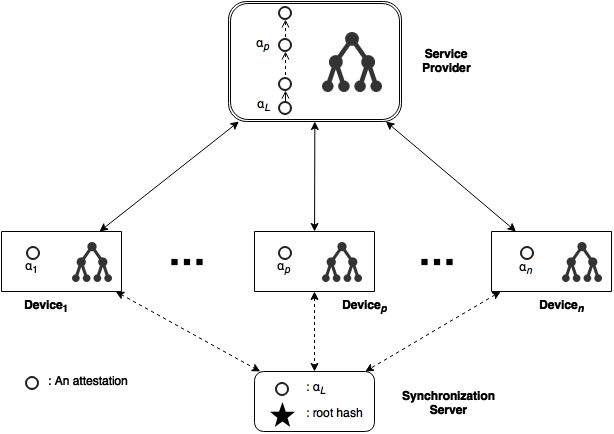
\includegraphics[width=.8\textwidth]{wei_shian}
	\end{center}
\end{frame}

\begin{frame}{Merkle Tree}
	\begin{center}
		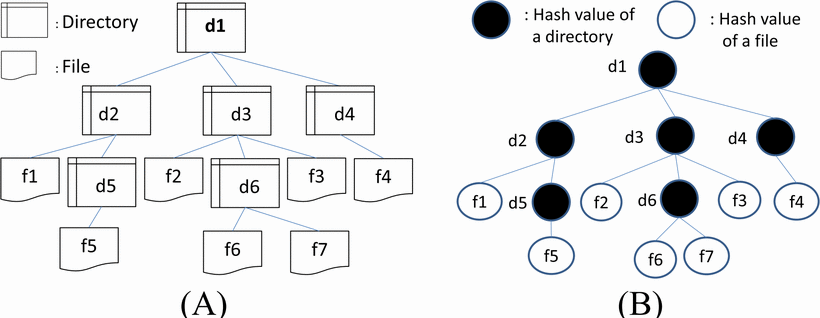
\includegraphics[width=.85\textwidth]{merkle_tree}
	\end{center}
\end{frame}

\begin{frame}{Worst-case}
	\textcolor{blue}{若有個 device 很久沒有使用,在讀寫檔案前需要更新大量未做的動作\\
	~\\
	使用者將會明顯感受到漫長的等待時間}\\
	~\\
	~\\
	~\\
	\begin{center}
		\includegraphics[width=.5\textwidth]{worst_case}
	\end{center}
\end{frame}

\subsection{\small{My Method}}
\begin{frame}{My Method}
	\textcolor{blue}{Assumption: $\text{同時有 k 個 server 上同一 file 出問題的機率} \approx 0$}
	\begin{center}
		\alert{Service Providers are Independent Cloud}
		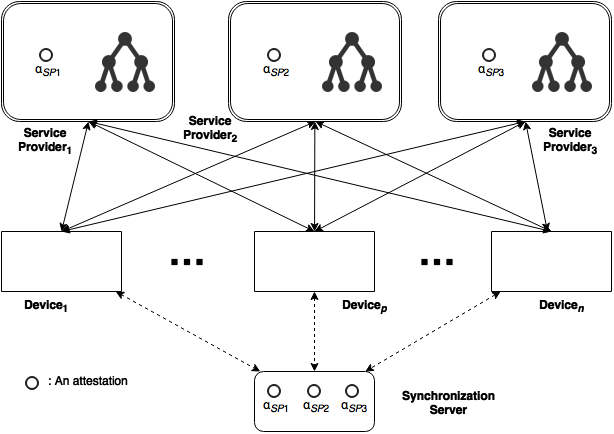
\includegraphics[width=.7\textwidth]{wei_chih}
	\end{center}
\end{frame}

\begin{frame}{Comparison}
	\begin{itemize}
		\item \textcolor{blue}{Pros}
			\begin{enumerate}
				\item Device 不用儲存、也不用修改 Merkle tree, 既省空間又省時間
				\item 資料有多份備份
				\item 解決之前的 Worst-case
			\end{enumerate}
		~\\
		\item \textcolor{red}{Cons}
			\begin{enumerate}
				\item 需要傳送多份 Request, 處理多份 Response
			\end{enumerate}
	\end{itemize}
\end{frame}
\section{Protocol Detail}

\subsection{Flowchart}
\begin{frame}{Flowchart}
	\begin{center}
		\resizebox{!}{.6\textwidth}
		{%
			\begin{tikzpicture}[node distance=2cm]
				% Define flow charts' component
				\node (init) [process] {Initial};
				\node (lock) [process, below of=init] {Lock};
				\node (twostep) [process, below of=lock] {2-step Handshake};
				\node (twostep_left) [process, left of=twostep, xshift=-2cm] {2-step Handshake};
				\node (twostep_right) [process, right of=twostep, xshift=2cm] {2-step Handshake};
				\node (voting) [decision, below of=twostep] {Voting};
				\node (store) [process, below of=voting, yshift=-0.5cm] {Store ACK};
				\node (update) [io, below of=store, align=center] {File \\ Transmit};
				\node (auditing) [process, right of=update, xshift=2.5cm] {Auditing};
				\node (unlock) [process, left of=store, xshift=-4cm] {Unlock};

				% Define flow charts' link
				\path [line](init) -- (lock);
				\path [line](lock) -- (twostep);
				\path [line](lock) -- (twostep_left);
				\path [line](lock) -- (twostep_right);
				\path [line](twostep) -- (voting);
				\path [line](twostep_left) -- (voting);
				\path [line](twostep_right) -- (voting);
				\path [line](voting) -- node[anchor=east] {k個以上的}
									    node[anchor=west] {ACK相同} (store);
				\path [line](voting) -| node[anchor=west] {ACK不相同} (auditing);
				\path [line](store) -- (update);
				\path [line](store) -- (unlock);
				\path [line](unlock) |- (lock);
			\end{tikzpicture}%
		}
	\end{center}
\end{frame}

\subsection{Download \& Upload}
\begin{frame}{Download \& Upload}
	\centering
	\textcolor{blue}{\textbf{Request \& Response}}\\
	~\\
	~\\
	\begin{minipage}{.45\textwidth}
        \includegraphics[width=1\textwidth]{2_step_handshake}
    \end{minipage}%
	\begin{minipage}{.55\textwidth}
    	\footnotesize
		\centering
		\begin{equation} \label{eq1}
                \begin{split}
                        \textcolor{blue}{REQ} & = (OP, [OP]_{pri(D)}) \\
                        OP & = (TYPE, PATH, HASH) \\
                \end{split}
        \end{equation}
        \divider{}\\
        \begin{equation} \label{eq2}
                \begin{split}
                        \textcolor{red}{ACK} & = (RESULT, REQ,\\
                        & \tab{}\tab{}[RESULT, REQ]_{pri(S)}) \\
                        RESULT & = (roothash, filehash)
                \end{split}
        \end{equation}
        \textcolor{red}{\textbf{collect ACKs and voting}}
    \end{minipage}%
\end{frame}

\begin{frame}{if Operation is UPLOAD}
	\centering
	\textcolor{blue}{\textbf{Server Update Merkle tree}}\\
	~\\
	~\\
	\begin{center}
		\includegraphics[width=.65\textwidth]{update_merkle_tree}
	\end{center}
\end{frame}

\begin{frame}{File Transmit}
	\begin{center}
		\includegraphics[width=.65\textwidth]{file_transmit}
	\end{center}
\end{frame}

\subsection{Audit}
\begin{frame}{Audit}
	\textcolor{blue}{$\because$ ACK 中有 roothash\\
	$\therefore$ 新的 request 之前,所有的檔案都經過檢查,沒有問題}\\
	~\\	
	\begin{block}{}
		\centering
		device request $OP_i$,收到回傳的 $ACK_i$\\
		發現 $Server_p$ 的 ACK 有錯誤,因此向 $Server_p$ 稽核\\
		~\\
		device 向 $Server_p$ 索取 $MT_{i-1}$\\
		($MT_{i-1}$ 為執行 $OP_i$ 之前的 Merkle tree)
	\end{block}
	\begin{alertblock}{\encircle{1}\encircle{2} 兩點有一個出錯就能確定 $Server_p$ 出錯}
		\encircle{1} device 檢查 $MT_{i-1}$ 的 roothash 應和 $ACK_{i-1}$ 中的 roothash 一樣\\
		\encircle{2} device 以 $OP_i$ 中的 hash value 來更新 $MT_{i-1}$,\\
		\tab{}更新後的 roothash 應和 $Server_p$ 現在的 roothash 相同
	\end{alertblock}	
\end{frame}
\section{Experimental Results}

\subsection{Generate Merkle tree}
\begin{frame}<beamer>
    \frametitle{Outline}
    \tableofcontents[currentsubsection]
\end{frame}

\begin{frame}{Experimental Results}
	\begin{table}[]
		\scriptsize
		\centering
		\begin{tabular}{crcc}
			  & Size    & File  & Directory \\
			  &			&		&		    \\
			A & 777 MB  & 48    & 6         \\
			B & 145 MB  & 54198 & 188       \\
			C & 5.95 GB & 45089 & 1459      \\
		\end{tabular}
        ~\\
        ~\\
        ~\\
		\caption{GENERATE MERKLE TREE'S TIME (IN SEC.)}
		\begin{tabular}{|c|c|c|r|}
			\hline
              & Non Hashed & Pre Hashed & Merkle tree Size \\ \hline
            A & 9.406    & 0.003    & 5.4 KB           \\ \hline
            B & 55.147   & 2.703    & 5.08 MB          \\ \hline
            C & 339.181  & 0.334    & 4.37 MB          \\ \hline
		\end{tabular}
        ~\\
        ~\\
        ~\\
        \caption{SERIALIZE \& DESERIALIZE MERKLE TREE OBJECT'S TIME (IN SEC.)}
		\begin{tabular}{|c|c|c|}
            \hline
              & Serialize & Deserialize \\ \hline
            A & 0.040      & 0.009       \\ \hline
            B & 0.756      & 0.299       \\ \hline
            C & 0.670      & 0.295       \\ \hline
		\end{tabular}
	\end{table}
\end{frame}

\subsection{Non POV}
\begin{frame}<beamer>
    \frametitle{Outline}
    \tableofcontents[currentsubsection]
\end{frame}

\begin{frame}{Experimental Results}{Non POV}
	\textcolor{blue}{not in the same network segment: from lab to my home (16 hops.)}\\
    \tiny
    \begin{table}[]
        \centering
        \begin{minipage}[c]{0.5\textwidth}
            \caption{The client device and SP are in the \newline same network segment}
            \begin{tabular}{lcc}
                                 & Upload (sec.) & Download (sec.) \\ \hline
                \textless 10 KB  & 0.010      & 0.007        \\ \hline
                \textless 100 KB & 0.014      & 0.013        \\ \hline
                \textless 1 MB   & 0.090      & 0.088        \\ \hline
                \textless 10 MB  & 0.367      & 0.354        \\ \hline
            \end{tabular}
            \begin{center}
                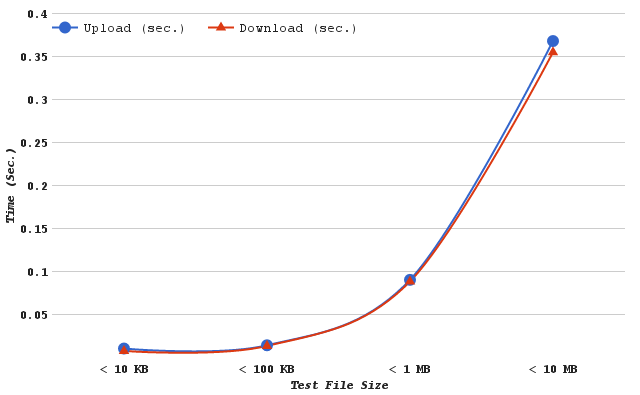
\includegraphics[width=\textwidth]{non_pov_same}
            \end{center}
        \end{minipage}%
        \begin{minipage}[c]{0.5\textwidth}
            \caption{The client device and SP are \alert{not} in the \newline same network segment}
            \begin{tabular}{lcc}
                                 & Upload (sec.) & Download (sec.) \\ \hline
                \textless 10 KB  & 0.069      & 0.056        \\ \hline
                \textless 100 KB & 0.121      & 0.087        \\ \hline
                \textless 1 MB   & 0.343      & 0.225        \\ \hline
                \textless 10 MB  & 1.675      & 0.699        \\ \hline
            \end{tabular}
            \begin{center}
                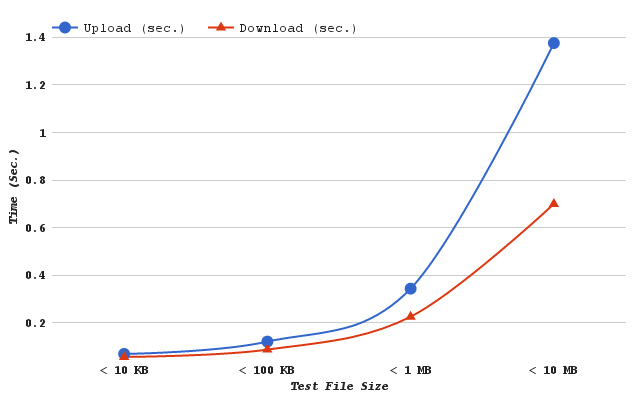
\includegraphics[width=\textwidth]{non_pov_not_same}
            \end{center}
        \end{minipage}
    \end{table}
\end{frame}

\subsection{Same Network Segment}
\begin{frame}<beamer>
    \frametitle{Outline}
    \tableofcontents[currentsubsection]
\end{frame}

\begin{frame}{Experimental Results}
{The client device and SP are in the same network segment - My Method}
	\scriptsize
    \begin{table}[]
    \centering
    \caption{THE EXECUTION TIME OF \alert{UPLOAD} OPERATIONS (IN SEC.) (Account C)}
    \begin{tabular}{lcccc}
                         & 3 Server & 5 Server & 7 Server & 9 Server \\ \hline
        \textless 10 KB  & 0.046 & 0.067 & 0.101 & 0.108 \\ \hline
        \textless 100 KB & 0.070 & 0.083 & 0.112 & 0.145 \\ \hline
        \textless 1 MB   & 0.153 & 0.166 & 0.200 & 0.203 \\ \hline
        \textless 10 MB  & 0.430 & 0.513 & 0.684 & 0.694 \\ \hline
    \end{tabular}
    \end{table}
    \begin{center}
		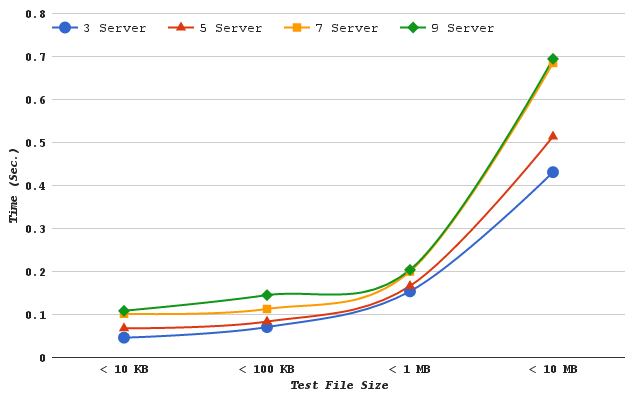
\includegraphics[width=.6\textwidth]{my_upload_same}
    \end{center}
\end{frame}

\begin{frame}{Experimental Results}
{The client device and SP are in the same network segment - My Method}
	\scriptsize
    \begin{table}[]
    \centering
    \caption{THE EXECUTION TIME OF \alert{DOWNLOAD} OPERATIONS (IN SEC.) (Account C)}
    \begin{tabular}{lcccc}
                         & 3 Server & 5 Server & 7 Server & 9 Server \\ \hline
        \textless 10 KB  & 0.042 & 0.054 & 0.064 & 0.078 \\ \hline
        \textless 100 KB & 0.053 & 0.055 & 0.083 & 0.097 \\ \hline
        \textless 1 MB   & 0.146 & 0.159 & 0.195 & 0.202 \\ \hline
        \textless 10 MB  & 0.392 & 0.476 & 0.622 & 0.625 \\ \hline
    \end{tabular}
    \end{table}
    \begin{center}
		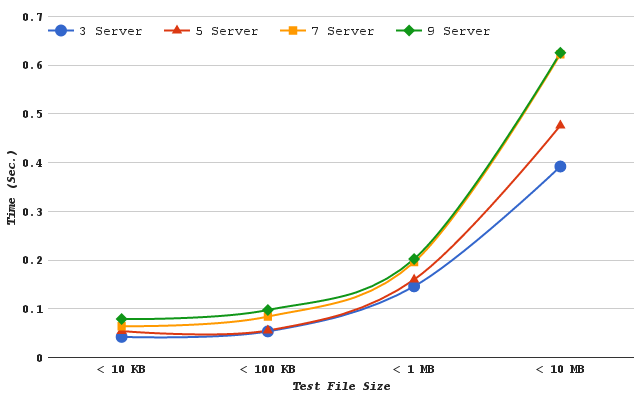
\includegraphics[width=.6\textwidth]{my_download_same}
    \end{center}
\end{frame}

\begin{frame}{Experimental Results}
{The client device and SP are in the same network segment - 2014 Cloud Com}
	\scriptsize
    \begin{table}[]
    \centering
    \caption{THE EXECUTION TIME OF \alert{UPLOAD} OPERATIONS (IN SEC.) (Account C)}
    \begin{tabular}{lccccl}
                         & sync 2   & sync 10  & sync 50  & sync 100 & sync 500 \\ \hline
        \textless 10 KB  & 0.146 & 0.184 & 0.332 & 0.409 & 0.760  \\ \hline
        \textless 100 KB & 0.194 & 0.209 & 0.341 & 0.491 & 0.932  \\ \hline
        \textless 1 MB   & 0.331 & 0.385 & 0.403 & 0.537 & 1.198  \\ \hline
        \textless 10 MB  & 0.501 & 0.518 & 0.576 & 0.819 & 1.242  \\ \hline
    \end{tabular}
    \end{table}
    \begin{center}
		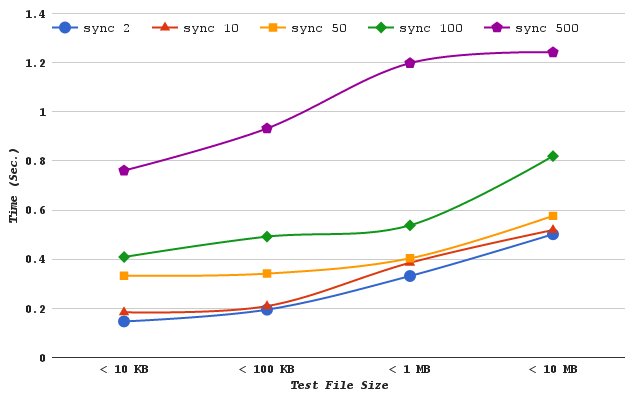
\includegraphics[width=.6\textwidth]{2014_upload_same}
    \end{center}
\end{frame}

\begin{frame}{Experimental Results}
{The client device and SP are in the same network segment - 2014 Cloud Com}
	\scriptsize
    \begin{table}[]
    \centering
    \caption{THE EXECUTION TIME OF \alert{DOWNLOAD} OPERATIONS (IN SEC.) (Account C)}
    \begin{tabular}{lccccl}
                         & sync 2   & sync 10  & sync 50  & sync 100 & sync 500  \\ \hline
        \textless 10 KB  & 0.121 & 0.249 & 0.331 & 0.515 & 1.675  \\ \hline
        \textless 100 KB & 0.134 & 0.258 & 0.338 & 0.564 & 1.796  \\ \hline
        \textless 1 MB   & 0.279 & 0.302 & 0.440 & 0.588 & 1.994  \\ \hline
        \textless 10 MB  & 0.462 & 0.539 & 0.595 & 1.171 & 2.241  \\ \hline
    \end{tabular}
    \end{table}
    \begin{center}
		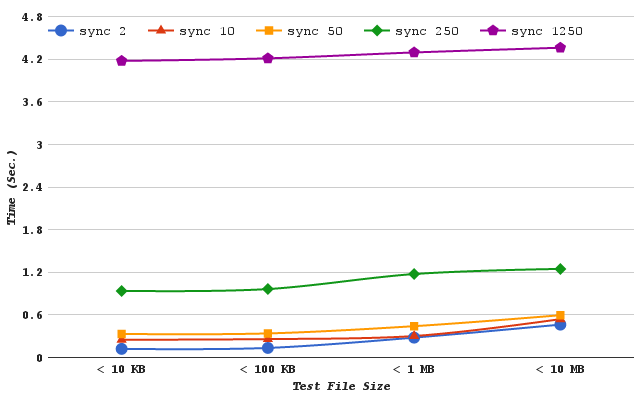
\includegraphics[width=.6\textwidth]{2014_download_same}
    \end{center}
\end{frame}

\begin{frame}{Experimental Results}
{The client device and SP are in the same network segment - UPLOAD operation}
	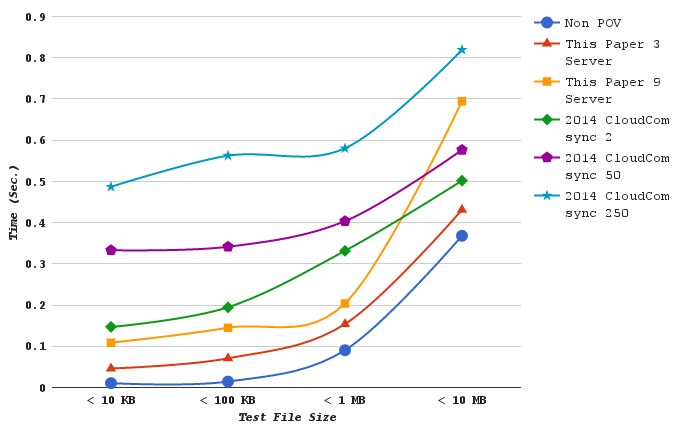
\includegraphics[width=\textwidth]{all_upload_same}
\end{frame}

\begin{frame}{Experimental Results}
{The client device and SP are in the same network segment - DOWNLOAD operation}
	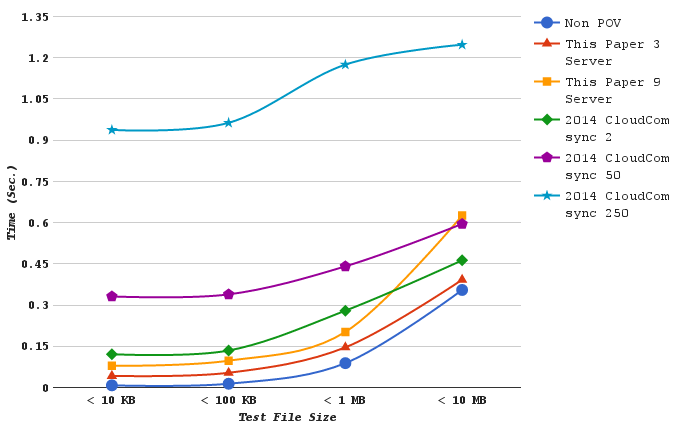
\includegraphics[width=\textwidth]{all_download_same}
\end{frame}

%TIMES
\begin{frame}{Experimental Results}
{The client device and SP are in the same network segment - UPLOAD Overhead}
	\scriptsize
    \begin{table}[]
    \centering
    \caption{My Method / Non POV (IN SEC.) (Account C)}
    \begin{tabular}{lcccc}
                         & 3 Server & 5 Server & 7 Server & 9 Server  \\ \hline
        \textless 10 KB  & 4.34 & 6.40 & 9.58 & 10.24 \\ \hline
        \textless 100 KB & 4.91 & 5.80 & 7.84 & 10.07 \\ \hline
        \textless 1 MB   & 1.70 & 1.83 & 2.21 & 2.25  \\ \hline
        \textless 10 MB  & 1.17 & 1.39 & 1.86 & 1.88  \\ \hline
    \end{tabular}
    \caption{2014 Cloud Com / Non POV (IN SEC.) (Account C)}
    \begin{tabular}{lccccl}
                         & sync 2    & sync 10   & sync 50   & sync 100 & sync 500 \\ \hline
        \textless 10 KB  & 13.83 & 17.35 & 31.39 & 38.55  & 71.72  \\ \hline
        \textless 100 KB & 13.52 & 14.52 & 23.72 & 34.18  & 64.75  \\ \hline
        \textless 1 MB   & 3.66  & 4.26  & 4.46  & 5.94   & 13.24  \\ \hline
        \textless 10 MB  & 1.36  & 1.40  & 1.56  & 2.22   & 3.37   \\ \hline
    \end{tabular}
    ~\\
    ~\\
    ~\\
    \alert{Avg: 3.97 times, Max: 6.99 times}
    \end{table}
\end{frame}

\begin{frame}{Experimental Results}
{The client device and SP are in the same network segment - DOWNLOAD Overhead}
	\scriptsize
    \begin{table}[]
    \centering
    \caption{My Method / Non POV (IN SEC.) (Account C)}
    \begin{tabular}{lcccc}
                         & 3 Server & 5 Server & 7 Server & 9 Server  \\ \hline
        \textless 10 KB  & 5.39 & 6.91 & 8.20 & 10.05 \\ \hline
        \textless 100 KB & 3.91 & 4.04 & 6.13 & 7.12  \\ \hline
        \textless 1 MB   & 1.64 & 1.80 & 2.21 & 2.28  \\ \hline
        \textless 10 MB  & 1.10 & 1.34 & 1.75 & 1.76  \\ \hline
    \end{tabular}
    \caption{2014 Cloud Com / Non POV (IN SEC.) (Account C)}
    \begin{tabular}{lccccl}
                         & sync 2    & sync 10   & sync 50   & sync 100   & sync 500  \\ \hline
        \textless 10 KB  & 15.45 & 31.84 & 42.23 & 119.48 & 532.25 \\ \hline
        \textless 100 KB & 9.82  & 18.89 & 24.74 & 70.34  & 307.57 \\ \hline
        \textless 1 MB   & 3.15  & 3.41  & 4.97  & 13.26  & 48.48  \\ \hline
        \textless 10 MB  & 1.30  & 1.52  & 1.67  & 3.51   & 12.28  \\ \hline
    \end{tabular}
    ~\\
    ~\\
    ~\\
    \alert{Avg: 7.91 times, Max: 21.24 times}
    \end{table}
\end{frame}

\subsection{Not Same Network Segment}
\begin{frame}<beamer>
    \frametitle{Outline}
    \tableofcontents[currentsubsection]
\end{frame}

\begin{frame}{Experimental Results}
{The client device and SP are \alert{not} in the same network segment - My Method}
	\scriptsize
    \begin{table}[]
    \centering
    \caption{THE EXECUTION TIME OF \alert{UPLOAD} OPERATIONS (IN SEC.) (Account C)}
    \begin{tabular}{lcccc}
                         & 3 Server & 5 Server & 7 Server & 9 Server \\ \hline
        \textless 10 KB  & 0.217 & 0.331 & 0.466 & 0.570 \\ \hline
        \textless 100 KB & 0.245 & 0.410 & 0.479 & 0.660 \\ \hline
        \textless 1 MB   & 0.433 & 0.594 & 0.640 & 0.786 \\ \hline
        \textless 10 MB  & 1.636 & 1.972 & 2.011 & 2.163 \\ \hline
    \end{tabular}
    \end{table}
    \begin{center}
		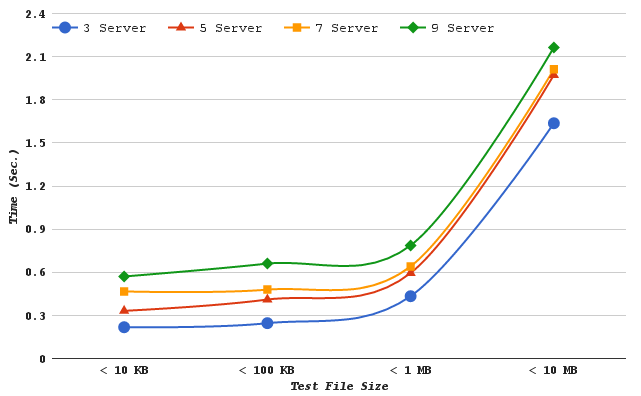
\includegraphics[width=.6\textwidth]{my_upload_not_same}
    \end{center}
\end{frame}

\begin{frame}{Experimental Results}
{The client device and SP are \alert{not} in the same network segment - My Method}
	\scriptsize
    \begin{table}[]
    \centering
    \caption{THE EXECUTION TIME OF \alert{DOWNLOAD} OPERATIONS (IN SEC.) (Account C)}
    \begin{tabular}{lcccc}
                         & 3 Server & 5 Server & 7 Server & 9 Server \\ \hline
        \textless 10 KB  & 0.263 & 0.358 & 0.490 & 0.556 \\ \hline
        \textless 100 KB & 0.270 & 0.396 & 0.567 & 0.597 \\ \hline
        \textless 1 MB   & 0.382 & 0.590 & 0.694 & 0.846 \\ \hline
        \textless 10 MB  & 0.823 & 1.086 & 1.208 & 1.278 \\ \hline
    \end{tabular}
    \end{table}
    \begin{center}
		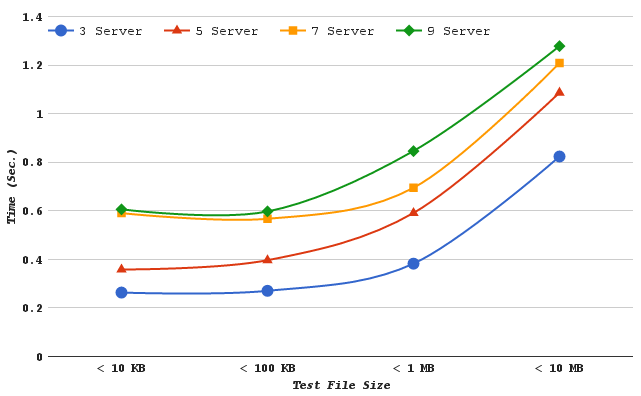
\includegraphics[width=.6\textwidth]{my_download_not_same}
    \end{center}
\end{frame}

\begin{frame}{Experimental Results}
{The client device and SP are \alert{not} in the same network segment - 2014 Cloud Com}
	\scriptsize
    \begin{table}[]
    \centering
    \caption{THE EXECUTION TIME OF \alert{UPLOAD} OPERATIONS (IN SEC.) (Account C)}
    \begin{tabular}{lccccl}
                         & sync 2   & sync 10  & sync 50  & sync 100 & sync 500  \\ \hline
        \textless 10 KB  & 0.362 & 0.411 & 0.486 & 0.500 & 1.227  \\ \hline
        \textless 100 KB & 0.377 & 0.416 & 0.508 & 0.563 & 1.375  \\ \hline
        \textless 1 MB   & 0.556 & 0.619 & 0.698 & 0.812 & 1.630  \\ \hline
        \textless 10 MB  & 1.525 & 1.882 & 1.929 & 1.962 & 2.753  \\ \hline
    \end{tabular}
    \end{table}
    \begin{center}
		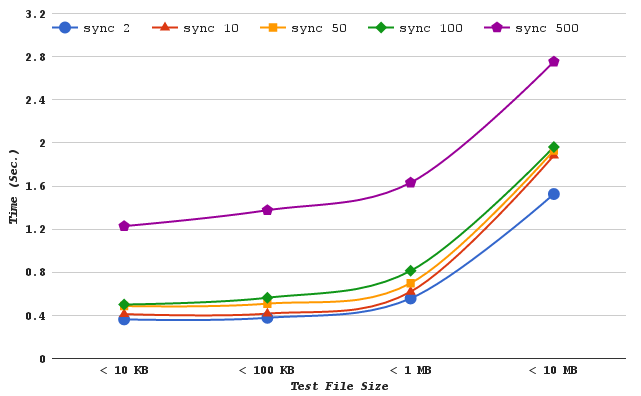
\includegraphics[width=.6\textwidth]{2014_upload_not_same}
    \end{center}
\end{frame}

\begin{frame}{Experimental Results}
{The client device and SP are \alert{not} in the same network segment - 2014 Cloud Com}
	\scriptsize
    \begin{table}[]
    \centering
    \caption{THE EXECUTION TIME OF \alert{DOWNLOAD} OPERATIONS (IN SEC.) (Account C)}
    \begin{tabular}{lccccl}
                         & sync 2   & sync 10  & sync 50  & sync 100 & sync 500  \\ \hline
        \textless 10 KB  & 0.388 & 0.374 & 0.524 & 0.646 & 2.269  \\ \hline
        \textless 100 KB & 0.427 & 0.440 & 0.584 & 0.735 & 2.302  \\ \hline
        \textless 1 MB   & 0.574 & 0.687 & 0.772 & 0.914 & 2.519  \\ \hline
        \textless 10 MB  & 0.933 & 1.024 & 1.145 & 1.414 & 2.884  \\ \hline
    \end{tabular}
    \end{table}
    \begin{center}
		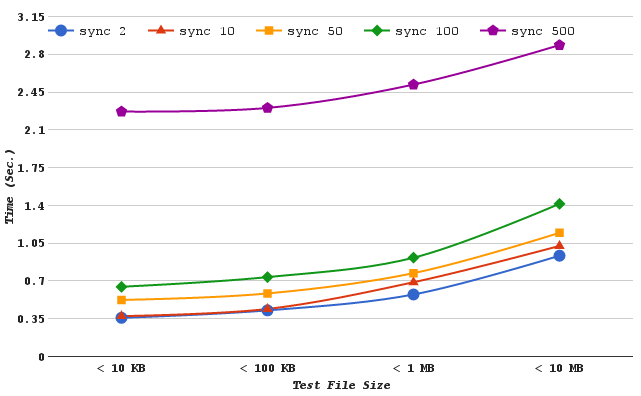
\includegraphics[width=.6\textwidth]{2014_download_not_same}
    \end{center}
\end{frame}

\begin{frame}{Experimental Results}
{The client device and SP are \alert{not} in the same network segment - UPLOAD operation}
	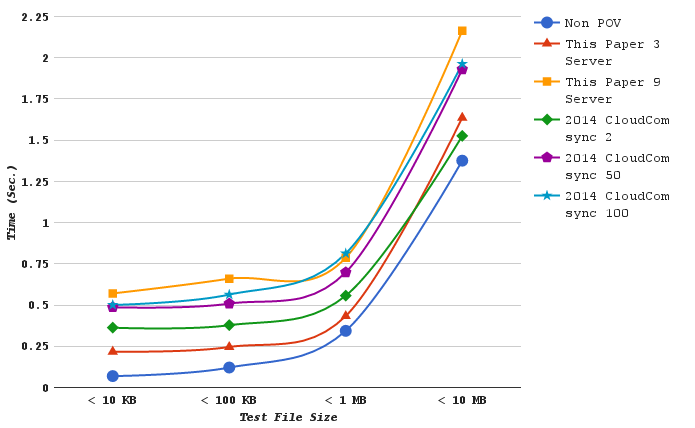
\includegraphics[width=\textwidth]{all_upload_not_same}
\end{frame}

\begin{frame}{Experimental Results}
{The client device and SP are \alert{not} in the same network segment - DOWNLOAD operation}
	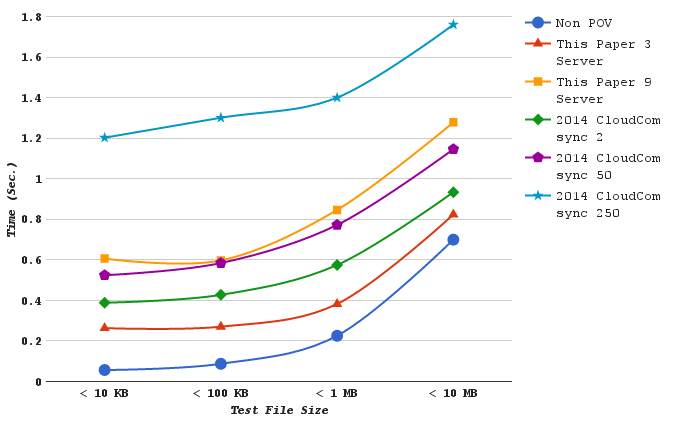
\includegraphics[width=\textwidth]{all_download_not_same}
\end{frame}

%TIMES
\begin{frame}{Experimental Results}
{The client device and SP are \alert{not} in the same network segment - UPLOAD Overhead}
	\scriptsize
    \begin{table}[]
    \centering
    \caption{My Method / Non POV (IN SEC.) (Account C)}
    \begin{tabular}{lcccc}
                         & 3 Server & 5 Server & 7 Server & 9 Server \\ \hline
        \textless 10 KB  & 3.14 & 4.78 & 6.73 & 8.23 \\ \hline
        \textless 100 KB & 2.02 & 3.38 & 3.95 & 5.45 \\ \hline
        \textless 1 MB   & 1.26 & 1.73 & 1.86 & 2.28 \\ \hline
        \textless 10 MB  & 1.18 & 1.43 & 1.46 & 1.57 \\ \hline
    \end{tabular}
    \caption{2014 Cloud Com / Non POV (IN SEC.) (Account C)}
    \begin{tabular}{lccccl}
                         & sync 2   & sync 10  & sync 50  & sync 100 & sync 500 \\ \hline
        \textless 10 KB  & 5.23 & 5.94 & 7.02 & 7.22   & 17.72  \\ \hline
        \textless 100 KB & 3.11 & 3.43 & 4.20 & 4.65   & 11.35  \\ \hline
        \textless 1 MB   & 1.62 & 1.80 & 2.03 & 2.36   & 4.74   \\ \hline
        \textless 10 MB  & 1.10 & 1.36 & 1.40 & 1.42   & 2.00   \\ \hline
    \end{tabular}
    ~\\
    ~\\
    ~\\
    \alert{Avg: 1.42 times, Max: 2.15 times}
    \end{table}
\end{frame}

\begin{frame}{Experimental Results}
{The client device and SP are \alert{not} in the same network segment - DOWNLOAD Overhead}
	\scriptsize
    \begin{table}[]
    \centering
    \caption{My Method / Non POV (IN SEC.) (Account C)}
    \begin{tabular}{lcccc}
                         & 3 Server & 5 Server & 7 Server & 9 Server \\ \hline
        \textless 10 KB  & 4.65 & 6.32 & 8.65 & 9.82 \\ \hline
        \textless 100 KB & 3.09 & 4.53 & 6.49 & 6.83 \\ \hline
        \textless 1 MB   & 1.69 & 2.62 & 3.07 & 3.75 \\ \hline
        \textless 10 MB  & 1.17 & 1.55 & 1.72 & 1.82 \\ \hline
    \end{tabular}
    \caption{2014 Cloud Com / Non POV (IN SEC.) (Account C)}
    \begin{tabular}{lccccl}
                         & sync 2   & sync 10  & sync 50  & sync 100 & sync 500 \\ \hline
        \textless 10 KB  & 6.86 & 6.60 & 9.25 & 11.41  & 40.07  \\ \hline
        \textless 100 KB & 4.89 & 5.04 & 6.68 & 8.41   & 26.36  \\ \hline
        \textless 1 MB   & 2.54 & 3.04 & 3.42 & 4.05   & 11.16  \\ \hline
        \textless 10 MB  & 1.33 & 1.46 & 1.63 & 2.02   & 4.12   \\ \hline
    \end{tabular}
    ~\\
    ~\\
    ~\\
    \alert{Avg: 1.88 times, Max: 4.08 times}
    \end{table}
\end{frame}
\section{Conclusion and Future Work}

\begin{frame}{Conclusion}
	我們提出了一個應用於雲端儲存的 Real-time POV 技術,利用投票的方式快速檢查 Data Integrity,也即時的將資料備份到多個 Server 上。\\
    ~\\
    ~\\
    實驗結果顯示,相較於之前的 Real-time POV 技術,平均能夠節省 8 倍的時間,Worst-case 時更能夠節省超過 20 倍的時間。\\
    ~\\
    ~\\
    雲端儲存系統可以使用本論文提出的方法,提供雙方不可否認的保證於他們的服務層級協議(Service Level Agreement)中。
\end{frame}

\begin{frame}{Future Work}
	\begin{enumerate}
		\item 我們希望能將 FBHTree\footnotemark 套用到本論文的方法中,藉由實驗觀察能否增快 Merkle tree 在更新檔案時的速度。\\
        ~\\
        \item 在本論文中使用同步伺服器來維護 Write Serializability,若有新的演算法能夠不需依賴同步伺服器又能維護 Write Serializability,將能讓我們的架構更加彈性且使用更少的硬體。
	\end{enumerate}
    \footnotetext{G.-H. Hwang and H.-F. Chen, "Efficient Real-time Auditing and Proof of Violation for Cloud Storage Systems," in 9th IEEE International Conference on Cloud Computing, San Francisco, USA, 2016.}
\end{frame}

\begin{frame}{Thanks for Your Listening}
	\begin{center}
		
\includegraphics[width=\textwidth]{thank_you.jpg}
	\end{center}	
\end{frame}

\end{CJK}
\end{document}